\chapter{Markov Chains}
\label{chap:markov-chains}

\section{First Examples and Definitions}
\label{sec:first-examples-definitions}

\subsection{Example 5.1}
\label{exm:telephone-markov}

In some homes the use of the telephone can become quite a sensitive issue. Suppose that if the phone is free during some period of time, say the $n$th minute, then with probability $p$, where $0 < p < 1$, it will be busy during the next minute. If the phone has been busy during the $n$th minute, it will become free during the next minute with probability $q$, where $0 < q < 1$. Assume that the phone is free in the 0th minute. We would like to answer the following two questions.

\begin{enumerate}
\item What is the probability $x_{n}$ that the telephone will be free in the $n$th minute?
\item What is $\lim_{n\to \infty}x_n$, if it exists?
\end{enumerate}

Denote by $A_{n}$ the event that the phone is free during the $n$th minute and let $B_{n} = \Omega \setminus A_{n}$ be its complement, i.e. the event that the phone is busy during the $n$th minute. The conditions of the example give us

\begin{align}
P(B_{n+1} | A_{n}) & = p, \tag{5.1} \\
P(A_{n+1} | B_{n}) & = q. \tag{5.2}
\end{align}

We also assume that $P(A_0) = 1$, i.e. $x_0 = 1$. Using this notation, we have $x_n = P(A_n)$. Then the total probability formula, see Exercise 1.10, together with (5.1)-(5.2) imply that

\begin{align}
x_{n+1} &= P(A_{n+1}) \tag{5.3} \\
&= P(A_{n+1} | A_{n}) P(A_{n}) + P(A_{n+1} | B_{n}) P(B_{n}) \\
&= (1-p) x_n + q(1-x_n) = q + (1-p-q) x_n.
\end{align}

It's a bit tricky to find an explicit formula for $x_n$. To do so we suppose first that the sequence $\{x_n\}$ is convergent, i.e.

\begin{align}
\lim_{n\to\infty} x_n = x. \tag{5.4}
\end{align}

The elementary properties of limits and equation (5.3), i.e. $x_{n+1} = q + (1-p-q)x_n$, yield

\begin{align}
x = q + (1-p-q)x. \tag{5.5}
\end{align}

The unique solution to the last equation is

\begin{align}
x = \frac{q}{q+p}. \tag{5.6}
\end{align}

In particular,

\begin{align}
\frac{q}{q+p} = q + (1-p-q)\frac{q}{q+p}. \tag{5.7}
\end{align}

Subtracting (5.7) from (5.3), we infer that

\begin{align}
x_{n+1} - \frac{q}{q+p} = (1-p-q)\left(x_n - \frac{q}{q+p}\right). \tag{5.8}
\end{align}

Thus, $\{x_n - \frac{q}{q+p}\}$ is a geometric sequence and therefore, for all $n\in\mathbb{N}$,

\begin{align}
x_n - \frac{q}{q+p} = (1-p-q)^n\left(x_0 - \frac{q}{q+p}\right).
\end{align}

Hence, by taking into account the initial condition $x_0 = 1$, we have

\begin{align}
x_n &= \frac{q}{q+p} + \left(x_0 - \frac{q}{q+p}\right)(1-p-q)^n \tag{5.9} \\
&= \frac{q}{q+p} + \frac{p}{q+p}(1-p-q)^n.
\end{align}

Let us point out that although we have used the assumption (5.4) to derive (5.8), the proof of the latter is now complete. Indeed, having proven (5.9), we can show that the assumption (5.4) is indeed satisfied. This is because the conditions $0 < p, q < 1$ imply that $|1-p-q| < 1$, and so $(1-p-q)^n \to 0$ as $n \to \infty$. Thus, (5.4) holds. This provides an answer to the second part of the example, i.e. $\lim_{n\to\infty} x_n = \frac{q}{p+q}$.

\begin{Exercise}
\label{exr:telephone-busy}
In the framework of Example \ref{exm:telephone-markov}, let $y_n$ denote the probability that the telephone is busy in the $n$th minute. Supposing that $y_0 = 1$, find an explicit formula for $y_n$ and, if it exists, $\lim_{n\to\infty} y_n$.

\begin{hint}
This exercise can be solved directly by repeating the above argument, or indirectly by using some of the results in Example \ref{exm:telephone-markov}.
\end{hint}
\end{Exercise}

\begin{Solution}
Since the telephone must be either free or busy at any time $n$, we have $x_n + y_n = 1$, where $x_n$ is the probability that the telephone is free. If $y_0 = 1$, then $x_0 = 0$. Substituting $x_0 = 0$ into the formula (5.9) for $x_n$ derived in Example \ref{exm:telephone-markov}, we obtain
\[
x_n = \frac{q}{q+p} + \left(0 - \frac{q}{q+p}\right)(1-p-q)^n = \frac{q}{q+p} - \frac{q}{q+p}(1-p-q)^n.
\]
Therefore,
\[
y_n = 1 - x_n = 1 - \frac{q}{q+p} + \frac{q}{q+p}(1-p-q)^n = \frac{p}{q+p} + \frac{q}{q+p}(1-p-q)^n.
\]
As $n \to \infty$, since $|1-p-q| < 1$, the term $(1-p-q)^n$ tends to zero, so
\[
\lim_{n\to\infty} y_n = \frac{p}{q+p}.
\]
\end{Solution}

\begin{Remark}
\label{rem:vector-matrix-form}
The formulae (5.3) and (5.9) can be written collectively in a compact form by using vector and matrix notation. First of all, since $x_n + y_n = 1$, we get

\begin{equation}
x_{n+1} = (1-p)x_n + q y_n,
\end{equation}

\begin{equation}
y_{n+1} = p x_n + (1-q) y_n.
\end{equation}

Hence, the matrix version takes the form

\begin{equation}
\begin{bmatrix}
x_{n+1} \\
y_{n+1}
\end{bmatrix}
=
\begin{bmatrix}
1-p & q \\
p & 1-q
\end{bmatrix}
\begin{bmatrix}
x_n \\
y_n
\end{bmatrix}.
\end{equation}

The situation described in Example \ref{exm:telephone-markov} is quite typical. Often the probability of a certain event at time $n+1$ depends only on what happens at time $n$, but not further into the past. Example \ref{exm:telephone-markov} provides us with a simple case of a Markov chain. See also the following definition and exercises.
\end{Remark}

\begin{Definition}[Markov chain]
\label{def:markov-chain}
Suppose that $S$ is a finite or a countable set. Suppose also that a probability space $(\Omega, \mathcal{F}, P)$ is given. An $S$-valued sequence of random variables $\xi_n$, $n\in\mathbb{N}$, is called an $S$-valued Markov chain or a Markov chain on $S$ if for all $n\in\mathbb{N}$ and all $s\in S$

\begin{align}
P(\xi_{n+1} = s \mid \xi_0, \dots, \xi_n) = P(\xi_{n+1} = s \mid \xi_n). \tag{5.10}
\end{align}

Here $P(\xi_{n+1}=s|\xi_n)$ is the conditional probability of the event $\{\xi_{n+1}=s\}$ with respect to random variable $\xi_n$, or equivalently, with respect to the $\sigma$-field $\sigma(\xi_n)$ generated by $\xi_n$. Similarly, $P(\xi_{n+1}=s|\xi_0,\ldots,\xi_n)$ is the conditional probability of $\{\xi_{n+1}=s\}$ with respect to the $\sigma$-field $\sigma(\xi_0,\cdots,\xi_n)$ generated by the random variables $\xi_0,\cdots,\xi_n$.

Property (5.10) will usually be referred to as the Markov property of the Markov chain $\xi_n, n\in\mathbb{N}$. The set $S$ is called the state space and the elements of $S$ are called states.
\end{Definition}

\begin{Proposition}
\label{prp:telephone-is-markov}
The model in Example \ref{exm:telephone-markov} and Exercise \ref{exr:telephone-busy} is a Markov chain.
\end{Proposition}

\begin{Proof}
Let $S = \{0,1\}$, where 0 and 1 represent the states of the phone being free or busy. First we need to construct an appropriate probability space. Let $\Omega$ be the set of all sequences $\omega_0, \omega_1, \ldots$ with values in $S$. Let $\mu_0$ be any probability measure on $S$. For example, $\mu = \delta_0$ corresponds to the case when the phone is free at time 0. We shall define $P$ by induction. For any $S$-valued sequence $s_0, s_1, \ldots$ we put

\begin{align}
P(\{\omega\in\Omega : \omega_0 = s_0\}) = \mu_0(\{s_0\}) \tag{5.11}
\end{align}

and

\begin{align}
&P(\{\omega\in\Omega : \omega_i = s_i, i=0,\ldots,n+1\}) \tag{5.12} \\
&= p(s_{n+1} \mid s_n) P(\{\omega\in\Omega : \omega_i = s_i, i=0,\ldots,n\}),
\end{align}

where $p(s \mid r)$ are the entries of the $2\times 2$ matrix

\begin{align}
\begin{bmatrix}
p(0 \mid 0) & p(0 \mid 1) \\
p(1 \mid 0) & p(1 \mid 1)
\end{bmatrix}
=
\begin{bmatrix}
1-p & q \\
p & 1-q
\end{bmatrix}.
\end{align}

It seems reasonable to expect $P$ to be a probability measure (with respect to the trivial $\sigma$-field of all subsets of $\Omega$). Take this for granted, check only that $P(\Omega) = 1$.

How would you define the process $\xi_n, n\in\mathbb{N}$? We shall do it in the standard way, i.e.

\begin{equation}
\xi_n(\omega) = \omega_n, \omega\in\Omega. \tag{5.13}
\end{equation}

First we shall show that the transition probabilities of $\xi_n$ are what they should be, i.e.

\begin{align}
P(\xi_{n+1} = 1 \mid \xi_n = 0) = p, \tag{5.14}
\end{align}

\begin{align}
P(\xi_{n+1} = 0 \mid \xi_n = 1) = q. \tag{5.15}
\end{align}

The definition of conditional probability yields

\begin{align}
P(\xi_{n+1} = 1 \mid \xi_n = 0) = \frac{P(\xi_{n+1} = 1, \xi_n = 0)}{P(\xi_n = 0)}.
\end{align}

Next, the definition of $P$ gives

\begin{equation}
\begin{aligned}
P(\xi_{n+1} = 1, \xi_n = 0)
&= P(\{\omega\in\Omega : \omega_n = 0, \omega_{n+1} = 1\}) \\
&= \sum_{s_0,\ldots,s_{n-1}\in S} P(\{\omega\in\Omega : \omega_i = s_i, i=0,\ldots,n-1, \omega_n = 0, \omega_{n+1} = 1\}) \\
&= \sum_{s_0,\ldots,s_{n-1}\in S} p P(\{\omega\in\Omega : \omega_i = s_i, i=0,\ldots,n-1, \omega_n = 0\}) \\
&= p P(\xi_n = 0),
\end{aligned}
\end{equation}

by (5.12). We have proven (5.14). Moreover, (5.15) follows by the same argument. A similar line of reasoning shows that $\xi_n$ is indeed a Markov chain. For this we need to verify that for any $n\in\mathbb{N}$ and any $s_0, s_1, \cdots, s_{n+1}\in S$

\begin{equation}
P(\xi_{n+1} = s_{n+1} \mid \xi_0 = s_0, \ldots, \xi_n = s_n) = P(\xi_{n+1} = s_{n+1} \mid \xi_n = s_n).
\end{equation}

We have

\begin{equation}
\begin{aligned}
&P(\xi_0 = s_0, \ldots, \xi_n = s_n, \xi_{n+1} = s_{n+1}) \\
&= P(\{\omega\in\Omega : \omega_i = s_i, i=0,\ldots,n+1\}) \\
&= p(s_{n+1} \mid s_n) P(\{\omega\in\Omega : \omega_i = s_i, i=0,\ldots,n\}) \\
&= p(s_{n+1} \mid s_n) P(\xi_0 = s_0, \ldots, \xi_n = s_n)
\end{aligned}
\end{equation}

which, in view of the definition of conditional probability, gives

\begin{equation}
P(\xi_{n+1} = s_{n+1} \mid \xi_0 = s_0, \ldots, \xi_n = s_n) = p(s_{n+1} \mid s_n).
\end{equation}

On the other hand, by an easy generalization of (5.14) and (5.15)

\begin{equation}
P(\xi_{n+1} = s_{n+1} \mid \xi_n = s_n) = p(s_{n+1} \mid s_n),
\end{equation}

which proves (5.10). \qed
\end{Proof}

In Example \ref{exm:telephone-markov} the transition probabilities from state $i$ to state $j$ do not depend on the time $n$. This is an important class of Markov chains.

\begin{Definition}[Time-homogeneous Markov chain]
\label{def:time-homogeneous}
An $S$-valued Markov chain $\xi_n, n\in\mathbb{N}$, is called time-homogeneous or homogeneous if for all $n\in\mathbb{N}$ and all $i, j\in S$

\begin{align}
P(\xi_{n+1} = j \mid \xi_n = i) = P(\xi_1 = j \mid \xi_0 = i). \tag{5.16}
\end{align}

The number $P(\xi_1 = j \mid \xi_0 = i)$ is denoted by $p(j \mid i)$ and called the transition probability from state $i$ to state $j$. The matrix $P = [p(j \mid i)]_{j,i\in S}$ is called the transition matrix of the chain $\xi_n$.
\end{Definition}

\begin{Exercise}
\label{exr:transition-matrix-columns}
In the discussion so far we have seen an example of a transition matrix, $P = \begin{bmatrix} 1-p & q \\ p & 1-q \end{bmatrix}$. Obviously the sum of the entries in each column of $P$ is equal to 1. Prove that this is true in general.

\begin{hint}
Remember that $P(\Omega \mid A) = 1$ for any event $A$.
\end{hint}
\end{Exercise}

\begin{Solution}
Let $P = [p(j \mid i)]_{j,i \in S}$ be a transition matrix, where $p(j \mid i) = P(\xi_{n+1} = j \mid \xi_n = i)$. The sum of the entries in the $i$-th column is given by
\[
\sum_{j \in S} p(j \mid i) = \sum_{j \in S} P(\xi_{n+1} = j \mid \xi_n = i) = P(\xi_{n+1} \in S \mid \xi_n = i).
\]
Since the random variable $\xi_{n+1}$ must take some value in the state space $S$, the event $\{\xi_{n+1} \in S\}$ is the entire sample space $\Omega$. Thus,
\[
\sum_{j \in S} p(j \mid i) = P(\Omega \mid \xi_n = i) = 1
\]
for any $i \in S$.
\end{Solution}

\begin{Definition}[Stochastic matrix]
\begin{enumerate}
\item the sum of the entries in each column is 1, i.e. $\sum_{j\in S} a_{ji} = 1$ for any $i\in S$.
\end{enumerate}

$A$ is called a double stochastic matrix if both $A$ and its transpose $A^t$ are stochastic matrices.
\end{Definition}

\begin{Proposition}
\label{prp:double-stochastic}
Show that a stochastic matrix is doubly stochastic if and only if the sum of the entries in each row is 1, i.e. $\sum_{i\in S} a_{ji} = 1$ for any $j\in S$.
\end{Proposition}

\begin{Solution}
By definition, a stochastic matrix $A$ is doubly stochastic if $A^t$ is also a stochastic matrix. Let $A = [a_{ji}]$. The sum of the entries in the $j$-th column of $A^t$ is equal to the sum of the entries in the $j$-th row of $A$:
\[
\sum_{i \in S} (A^t)_{ij} = \sum_{i \in S} a_{ji}.
\]
If $A$ is doubly stochastic, this sum must be 1 for all $j \in S$. Conversely, if $\sum_{i \in S} a_{ji} = 1$ for all $j \in S$, then $A^t$ is a stochastic matrix (since its columns sum to 1 and its entries are non-negative), which means $A$ is doubly stochastic.
\end{Solution}

\begin{Exercise}
\label{exr:power-of-stochastic}
Show that if $P = [p_{ji}]_{j,i\in S}$ is a stochastic matrix, then any natural power $P^n$ of $P$ is a stochastic matrix. Is the corresponding result true for a double stochastic matrix?

\begin{hint}
Show that if $A$ and $B$ are two stochastic matrices, then so is $BA$. For the second problem, recall that $(BA)^t = A^t B^t$.
\end{hint}
\end{Exercise}

\begin{Solution}
Let $A$ and $B$ be two stochastic matrices. Let $C = BA$. The entries of $C$ are $c_{ji} = \sum_k b_{jk} a_{ki}$. Since $a_{ki} \geq 0$ and $b_{jk} \geq 0$, it follows that $c_{ji} \geq 0$. The sum of the entries in each column of $C$ is
\[
\sum_j c_{ji} = \sum_j \sum_k b_{jk} a_{ki} = \sum_k a_{ki} \left( \sum_j b_{jk} \right) = \sum_k a_{ki} \cdot 1 = 1,
\]
where we used the fact that $B$ is stochastic ($\sum_j b_{jk} = 1$) and $A$ is stochastic ($\sum_k a_{ki} = 1$). Thus $BA$ is stochastic. By induction, if $P$ is stochastic, then $P^n = P \cdot P^{n-1}$ is stochastic for all $n \in \mathbb{N}$.

If $P$ is doubly stochastic, then $P$ and $P^t$ are both stochastic. From the result above, $P^n$ is stochastic. Also, $(P^n)^t = (P^t)^n$ is a product of stochastic matrices ($P^t$), so $(P^n)^t$ is also stochastic. Thus $P^n$ is doubly stochastic.
\end{Solution}

\begin{Exercise}
\label{exr:compute-p-squared}
Let $P = \begin{bmatrix} 1-p & q \\ p & 1-q \end{bmatrix}$. Show that

\begin{align}
P^2 = \begin{bmatrix}
1+p^2-2p+pq & 2q-pq-q^2 \\
2p-pq-p^2 & 1+q^2-2q+pq
\end{bmatrix}.
\end{align}

\begin{hint}
This is just simple matrix multiplication.
\end{hint}
\end{Exercise}

\begin{Solution}
Using matrix multiplication, we have
\begin{align*}
P^2 &= \begin{bmatrix} 1-p & q \\ p & 1-q \end{bmatrix} \begin{bmatrix} 1-p & q \\ p & 1-q \end{bmatrix} \\
&= \begin{bmatrix} (1-p)^2 + qp & (1-p)q + q(1-q) \\ p(1-p) + (1-q)p & pq + (1-q)^2 \end{bmatrix} \\
&= \begin{bmatrix} 1-2p+p^2+pq & q-pq+q-q^2 \\ p-p^2+p-pq & pq+1-2q+q^2 \end{bmatrix} \\
&= \begin{bmatrix} 1+p^2-2p+pq & 2q-pq-q^2 \\ 2p-pq-p^2 & 1+q^2-2q+pq \end{bmatrix}.
\end{align*}
\end{Solution}

We see that there is a problem with finding higher powers of the matrix $P$. When multiplying $P^2$ by $P$, $P^3$, and so on, we obtain more and more complicated expressions.

\begin{Definition}[$n$-step transition matrix]
\label{def:n-step-transition}
The $n$-step transition matrix of a Markov chain $\xi_n$ with transition probabilities $p(j \mid i)$, $j, i\in S$ is the matrix $P_n$ with entries

\begin{equation}
p_n(j \mid i) = P(\xi_n = j \mid \xi_0 = i). \tag{5.17}
\end{equation}
\end{Definition}

\begin{Exercise}
\label{exr:find-n-step-transition}
Find an exact formula for $P_n$ for the matrix $P$ from Exercise \ref{exr:compute-p-squared}.

\begin{hint}
Put $x_n = P(\xi_n = 0 \mid \xi_0 = 0)$ and $y_n = P(\xi_n = 1 \mid \xi_0 = 1)$. Is it correct to suppose that $p_n(0 \mid 0) = x_n$ and $p_n(1 \mid 1) = y_n$? If yes, you may be able use Example \ref{exm:telephone-markov} and Exercise \ref{exr:telephone-busy}.
\end{hint}
\end{Exercise}

\begin{Solution}
The entries of $P_n$ are $p_n(j \mid i) = P(\xi_n = j \mid \xi_0 = i)$. 
From Example \ref{exm:telephone-markov}, if $\xi_0 = 0$ (phone is free), the probability that $\xi_n = 0$ is $x_n$ given by (5.9):
\[
p_n(0 \mid 0) = \frac{q}{q+p} + \frac{p}{q+p}(1-p-q)^n.
\]
Then $p_n(1 \mid 0) = 1 - p_n(0 \mid 0) = \frac{p}{q+p} - \frac{p}{q+p}(1-p-q)^n$.
From Exercise \ref{exr:telephone-busy}, if $\xi_0 = 1$ (phone is busy), the probability that $\xi_n = 1$ is $y_n$:
\[
p_n(1 \mid 1) = \frac{p}{q+p} + \frac{q}{q+p}(1-p-q)^n.
\]
Then $p_n(0 \mid 1) = 1 - p_n(1 \mid 1) = \frac{q}{q+p} - \frac{q}{q+p}(1-p-q)^n$.
Thus, the $n$-step transition matrix is
\[
P_n = \frac{1}{q+p} \begin{bmatrix} q+p(1-p-q)^n & q-q(1-p-q)^n \\ p-p(1-p-q)^n & p+q(1-p-q)^n \end{bmatrix}.
\]
\end{Solution}

\begin{Exercise}
\label{exr:pn-equals-p-power}
You may suspect that $P_n$ equals $P^n$, the $n$th power of the matrix $P$. This holds for $n=1$. Check if it is true for $n=2$. If this is the case, try to prove that $P_n = P^n$ for all $n\in\mathbb{N}$.

\begin{hint}
Once again, this is an exercise in matrix multiplication.
\end{hint}
\end{Exercise}

\begin{Solution}
For $n=2$, $p_2(j \mid i) = P(\xi_2 = j \mid \xi_0 = i)$. By the law of total probability,
\[
p_2(j \mid i) = \sum_{k \in S} P(\xi_2 = j \mid \xi_1 = k, \xi_0 = i) P(\xi_1 = k \mid \xi_0 = i).
\]
By the Markov property, $P(\xi_2 = j \mid \xi_1 = k, \xi_0 = i) = P(\xi_2 = j \mid \xi_1 = k) = p(j \mid k)$. Thus,
\[
p_2(j \mid i) = \sum_{k \in S} p(j \mid k) p(k \mid i),
\]
which are the entries of $P^2$. So $P_2 = P^2$.
By induction, assume $P_n = P^n$. Then
\[
p_{n+1}(j \mid i) = \sum_{k \in S} P(\xi_{n+1} = j \mid \xi_n = k, \xi_0 = i) P(\xi_n = k \mid \xi_0 = i) = \sum_{k \in S} p(j \mid k) p_n(k \mid i).
\]
In matrix notation, this is $P_{n+1} = P P_n = P P^n = P^{n+1}$.
\end{Solution}

The following is a generalization of Exercise \ref{exr:pn-equals-p-power}.

\begin{Proposition}[Chapman--Kolmogorov equation]
\label{prp:chapman-kolmogorov}
Suppose that $\xi_n, n\in\mathbb{N}$, is an $S$-valued Markov chain with $n$-step transition probabilities $p_n(j \mid i)$. Then for all $k, n\in\mathbb{N}$

\begin{align}
p_{n+k}(j \mid i) = \sum_{s\in S} p_n(j \mid s) p_k(s \mid i), \quad i,j\in S. \tag{5.18}
\end{align}
\end{Proposition}

\begin{Exercise}
\label{exr:prove-chapman-kolmogorov}
Prove Proposition \ref{prp:chapman-kolmogorov}.

\begin{hint}
$p_{n+k}(j \mid i)$ are the entries of the matrix $P_{n+k} = P^{n+k}$.
\end{hint}
\end{Exercise}

\begin{Solution}
The $n$-step transition probabilities $p_m(j \mid i)$ are the entries of the matrix $P_m = P^m$. The Chapman-Kolmogorov equation
\[
p_{n+k}(j \mid i) = \sum_{s \in S} p_n(j \mid s) p_k(s \mid i)
\]
is equivalent to the matrix identity
\[
P_{n+k} = P_n P_k.
\]
Since $P_m = P^m$, we have $P_{n+k} = P^{n+k} = P^n P^k = P_n P_k$, which proves the proposition.
\end{Solution}

\begin{Exercise}
\label{exr:random-walk}
Suppose that $S = \mathbb{Z}$. Let $\eta_n, n \geq 1$ be a sequence of independent identically distributed random variables with $P(\eta_1 = 1) = p$ and $P(\eta_1 = -1) = q = 1-p$. Define $\xi_n = \sum_{i=1}^n \eta_i$ for $n \geq 1$ and $\xi_0 = 0$. Show that $\xi_n$ is a Markov chain with transition probabilities

\begin{align}
p(j \mid i) = \begin{cases}
p, & \text{if } j = i+1, \\
q, & \text{if } j = i-1, \\
0, & \text{otherwise}.
\end{cases}
\end{align}

$\xi_n, n \geq 0$, is called a random walk starting at 0. Replacing $\xi_0 = 0$ with $\xi_0 = i$, we get a random walk starting at $i$.

\begin{hint}
$\xi_{n+1} = \xi_n + \eta_{n+1}$. Are $\xi_n$ and $\eta_{n+1}$ independent?
\end{hint}
\end{Exercise}

\begin{Solution}
We have $\xi_{n+1} = \xi_n + \eta_{n+1}$. Since $\eta_{n+1}$ is independent of $\eta_1, \dots, \eta_n$, it is independent of $\xi_0, \dots, \xi_n$. Thus,
\begin{align*}
P(\xi_{n+1} = j \mid \xi_n = i, \xi_{n-1} = s_{n-1}, \dots, \xi_0 = s_0) &= P(\xi_n + \eta_{n+1} = j \mid \xi_n = i, \dots, \xi_0 = s_0) \\
&= P(i + \eta_{n+1} = j \mid \xi_n = i, \dots, \xi_0 = s_0) \\
&= P(\eta_{n+1} = j - i).
\end{align*}
Since this depends only on $i$, the chain is Markov. The transition probabilities are
\[
p(j \mid i) = P(\eta_{n+1} = j - i) = \begin{cases} p & \text{if } j-i=1 \Rightarrow j=i+1 \\ q & \text{if } j-i=-1 \Rightarrow j=i-1 \\ 0 & \text{otherwise} \end{cases}
\]
which is what we wanted to show.
\end{Solution}

\begin{Exercise}
\label{exr:random-walk-binomial}
For the random walk $\xi_n$ defined in Exercise \ref{exr:random-walk} prove that

\begin{equation}
P(\xi_n = j \mid \xi_0 = i) = \binom{n}{\frac{n+j-i}{2}} p^{\frac{n+j-i}{2}} q^{\frac{n-j+i}{2}} \tag{5.19}
\end{equation}

if $n+j-i$ is an even non-negative integer, and $P(\xi_n = j \mid \xi_0 = i) = 0$ otherwise.

\begin{hint}
Use induction. Note that $\binom{n}{\frac{n+j-i}{2}}p^{\frac{n+j-i}{2}}$ equals 0 if $|j-i| \geq n+1$.
\end{hint}
\end{Exercise}

\begin{Solution}
Let $k$ be the number of steps to the right ($+1$) and $m$ be the number of steps to the left ($-1$) in $n$ trials. Then $k+m=n$. The displacement is $\xi_n - \xi_0 = k - m = k - (n - k) = 2k - n$.
We want to find $P(\xi_n = j \mid \xi_0 = i)$, which is the probability that $2k - n = j - i$, or $2k = n + j - i$.
This gives $k = \frac{n+j-i}{2}$ and $m = n - k = \frac{n-j+i}{2}$.
For such $k$ and $m$ to exist, $n+j-i$ must be an even integer between 0 and $2n$.
Since the steps are independent and have the same distribution, the number of steps to the right follows a binomial distribution $B(n, p)$. Thus,
\[
P(\xi_n = j \mid \xi_0 = i) = P(k \text{ steps to the right}) = \binom{n}{k} p^k q^{n-k} = \binom{n}{\frac{n+j-i}{2}} p^{\frac{n+j-i}{2}} q^{\frac{n-j+i}{2}}.
\]
If $n+j-i$ is odd, or if $k < 0$ or $k > n$, it is impossible to reach state $j$ from $i$ in $n$ steps, so the probability is 0.
\end{Solution}

\begin{Proposition}
\label{prp:simple-random-walk-return-prob}
For all $p \in (0,1)$
\[
P(\xi_n = i \mid \xi_0 = i) \to 0 \quad \text{as } n \to \infty. \tag{5.20}
\]
\end{Proposition}

\begin{Proof}
To begin with, we shall consider the case $p \neq \frac{1}{2}$. When $j = i$, formula (5.19) becomes
\[
P(\xi_n = i \mid \xi_0 = i) = \begin{cases} \frac{(2k)!}{(k!)^2} (pq)^k, & \text{if } n = 2k, \\ 0, & \text{if } n \text{ is odd.} \end{cases} \tag{5.21}
\]

Then, denoting $a_k = \frac{(2k)!}{(k!)^2} (pq)^k$, we have
\[
\frac{a_{k+1}}{a_k} = pq \frac{(2k+1)(2k+2)}{(k+1)^2} \to 4pq < 1.
\]

Hence, $a_k \to 0$. Thus, $P(\xi_{2k} = i \mid \xi_0 = i) \to 0$. The result follows, since $P(\xi_{2k+1} = i \mid \xi_0 = i) = 0 \to 0$.

This argument does not work for $p = \frac{1}{2}$ because $4pq = 1$. In this case we shall need the Stirling formula
\[
k! \sim \sqrt{2\pi k} \left(\frac{k}{e}\right)^k \quad \text{as } k \to \infty. \tag{5.22}
\]

Here we use the standard convention: $a_n \sim b_n$ whenever $\frac{a_n}{b_n} \to 1$ as $n \to \infty$. By (5.22)
\[
a_k \sim \frac{\sqrt{4\pi k}}{2\pi k} \left(\frac{2k}{e}\right)^{2k} \left(\frac{e}{k}\right)^{2k} (pq)^k = \frac{1}{\sqrt{\pi k}} \to 0 \quad \text{as } k \to \infty.
\]

Let us note that the second method works in the first case too. However, in the first case there is no need for anything as sophisticated as the Stirling formula. $\square$
\end{Proof}

\begin{Proposition}
\label{prp:return-probability}
The probability that the random walk $\xi_n$ ever returns to the starting point is
\[
1 - |p - q|.
\]
\end{Proposition}

\begin{Proof}
Suppose that $\xi_0 = 0$ and denote by $f_0(n)$ the probability that the process returns to $0$ at time $n$ for the first time, i.e.
\[
f_0(n) = P(\xi_n = 0, \xi_i \neq 0, i = 1, \dots, n-1).
\]

If also $p_0(n) = P(\xi_n = 0)$ for any $n \in \mathbb{N}$, then we can prove that
\[
\sum_{n=1}^\infty p_0(n) = \sum_{n=0}^\infty p_0(n) \sum_{n=1}^\infty f_0(n). \tag{5.23}
\]

Since all the numbers involved are non-negative, in order to prove (5.23) we need only to show that
\[
p_0(n) = \sum_{k=1}^n f_0(k) p_0(n-k) \quad \text{for } n \geq 1.
\]

The total probability formula and the Markov property (5.10) yield
\[
\begin{aligned}
p_0(n) &= \sum_{k=1}^n P(\xi_n = 0, \xi_k = 0, \xi_i \neq 0, i = 1, \dots, k-1) \\
&= \sum_{k=1}^n P(\xi_k = 0, \xi_i \neq 0, i = 1, \dots, k-1) \\
&\quad \times P(\xi_n = 0 \mid \xi_k = 0, \xi_i \neq 0, i = 1, \dots, k-1) \\
&= \sum_{k=1}^n P(\xi_k = 0, \xi_i \neq 0, i = 1, \dots, k-1) P(\xi_n = 0 \mid \xi_k = 0) \\
&= \sum_{k=1}^n f_0(k) p_0(n-k).
\end{aligned}
\]

Having proved (5.23), we are going to make use of it. First we notice that the probability that the process will ever return to $0$ equals $\sum_{n=1}^\infty f_0(n)$. Next, from (5.23) we infer that
\[
\begin{aligned}
P(\exists n \geq 1: \xi_n = 0) &= \sum_{n=1}^\infty f_0(n) \\
&= 1 - \left(\sum_{n=0}^\infty p_0(n)\right)^{-1} = 1 - \left(\sum_{k=0}^\infty p_0(2k)\right)^{-1}.
\end{aligned}
\]

Since $p_0(2k) = \frac{(2k)!}{(k!)^2} (pq)^k$ and
\[
\sum_{k=0}^\infty \binom{2k}{k} x^k = (1-4x)^{-1/2}, \quad |x| < \frac{1}{4}, \tag{5.24}
\]
it follows that for $p \neq 1/2$
\[
P(\exists n \geq 1: \xi_n = 0) = 1 - (1-4pq)^{1/2} = 1 - |p - q|, \tag{5.25}
\]
since, recalling that $q = 1-p$, we have $1-4pq = 1-4p+4p^2 = (1-2p)^2 = (q-p)^2$.

The case $p = 1/2$ is more delicate and we shall not pursue this topic here. $\square$
\end{Proof}

\begin{Exercise}
\label{exr:binomial-series}
Prove formula (5.24).

\begin{hint}
Use the Taylor formula to expand the right-hand side of (5.24) into a power series.
\end{hint}
\end{Exercise}

\begin{Solution}
Assuming (5.24) refers to the generating function for the return probabilities $P_{ii}(x) = (1 - 4pqx^2)^{-1/2}$, we use the binomial series expansion:
\[
(1-z)^{-1/2} = \sum_{k=0}^\infty \binom{-1/2}{k} (-z)^k = \sum_{k=0}^\infty \frac{(-1/2)(-3/2)\cdots(-(2k-1)/2)}{k!} (-z)^k.
\]
This simplifies to
\[
(1-z)^{-1/2} = \sum_{k=0}^\infty \frac{1 \cdot 3 \cdot \cdots \cdot (2k-1)}{2^k k!} z^k = \sum_{k=0}^\infty \frac{(2k)!}{2^{2k} (k!)^2} z^k = \sum_{k=0}^\infty \binom{2k}{k} \left(\frac{z}{4}\right)^k.
\]
Setting $z = 4pqx^2$, we obtain
\[
P_{ii}(x) = \sum_{k=0}^\infty \binom{2k}{k} (pqx^2)^k = \sum_{k=0}^\infty \binom{2k}{k} p^k q^k x^{2k}.
\]
Comparing this with $P_{ii}(x) = \sum_n p_n(i \mid i) x^n$, we see that $p_{2k}(i \mid i) = \binom{2k}{k} p^k q^k$ and $p_{2k+1}(i \mid i) = 0$, which is consistent with the formula derived in Exercise \ref{exr:random-walk-binomial}.
\end{Solution}

\begin{Exercise}[Branching process]
\label{exr:branching-process}
On the island Elschenbieden there lives an almost extinct species called Vugiel. Vugiel's males can produce zero, one, two, $\cdots$ male offspring with probability $p_0, p_1, p_2, \cdots$ respectively, where $p_i \geq 0$ and $\sum_{i=0}^\infty p_i = 1$. A challenging problem would be to find the Vugiel's chances of survival assuming that each individual lives exactly one year. At this moment, we ask you only to rewrite the problem in the language of Markov chains.

\begin{hint}
The number of descendants of each male has the same distribution.
\end{hint}
\end{Exercise}

\begin{Solution}
Let $\xi_n$ be the number of males in the $n$-th generation. Since each individual lives for exactly one year and produces offspring at the end of that year, the population at time $n+1$ consists entirely of the offspring of the population at time $n$. Thus,
\[
\xi_{n+1} = \sum_{j=1}^{\xi_n} X_j^{(n)},
\]
where $X_j^{(n)}$ is the number of offspring produced by the $j$-th individual of the $n$-th generation. The random variables $X_j^{(n)}$ are independent and identically distributed with $P(X_j^{(n)} = k) = p_k$. If $\xi_n = 0$, the sum is empty and we define $\xi_{n+1} = 0$, meaning the species is extinct. The process $\xi_n$ is a Markov chain on the state space $S = \{0, 1, 2, \dots\}$ with transition probabilities
\[
p(j \mid i) = P\left( \sum_{k=1}^i X_k = j \right),
\]
where $X_k$ are independent random variables each with the offspring distribution $\{p_k\}$.
\end{Solution}

\begin{Exercise}
\label{exr:branching-binomial-poisson}
Consider the following two cases:

\begin{enumerate}
\item In Exercise \ref{exr:branching-process} suppose that

\begin{equation}
p_m = \binom{N}{m} p^m (1-p)^{N-m}.
\end{equation}

for some $p\in(0,1)$ and $N\in\mathbb{N}^*$, where $\mathbb{N}^* = \{1,2,3,\cdots\}$. (Note that $p_m = 0$ if $m > N$.) Show that

\begin{align}
p(j \mid i) = \binom{Ni}{j} p^j (1-p)^{Ni-j}. \tag{5.26}
\end{align}

Deduce that, in particular, $p(j \mid i) = 0$ if $j > Ni$.

\item Suppose that

\begin{align}
p_m = \frac{\lambda^m}{m!} e^{-\lambda}, m\in\mathbb{N},
\end{align}

for some $\lambda > 0$. In other words, assume that each $X_j$ has the Poisson distribution with mean $\lambda$. Show that

\begin{equation}
p(j \mid i) = \frac{(\lambda i)^j}{j!} e^{-\lambda i}, j,i \geq 0. \tag{5.27}
\end{equation}
\end{enumerate}

\begin{hint}
If $X_1$ has the binomial distribution $P(X_1=m) = \binom{N}{m}p^m(1-p)^{N-m}, m\in\mathbb{N}$, then there exists a finite sequence $\eta_1^1, \cdots, \eta_N^1$ of independent identically distributed random variables such that $P(\eta_j^1 = 1) = p$, $P(\eta_j^1 = 0) = 1-p$ and $X_j = \eta_1^j + \cdots + \eta_N^j = m$. Hence, $X_1 + \cdots + X_i = \sum_{r=1}^i \sum_{s=1}^N \eta_s^r$, i.e. the sum of $Ni$ independent identically distributed random variables with distribution as above. Hence we infer (5.26).
\end{hint}
\end{Exercise}

\begin{Solution}
\begin{enumerate}
\item The number of offspring $X_k$ of each individual has the binomial distribution $B(N, p)$. The transition probability $p(j \mid i)$ is the probability that the sum of $i$ such independent variables is $j$. Since the sum of $i$ independent $B(N, p)$ variables is a $B(Ni, p)$ variable, we have
\[
p(j \mid i) = P\left( \sum_{k=1}^i X_k = j \right) = \binom{Ni}{j} p^j (1-p)^{Ni-j}.
\]
Clearly, if $j > Ni$, then $p(j \mid i) = 0$.
\item If each $X_k$ has the Poisson distribution with mean $\lambda$, then the sum of $i$ independent such variables has the Poisson distribution with mean $i\lambda$. Thus,
\[
p(j \mid i) = P\left( \sum_{k=1}^i X_k = j \right) = \frac{(i\lambda)^j}{j!} e^{-i\lambda}.
\]
\end{enumerate}
\end{Solution}

\begin{Proposition}
\label{prp:survival-probability}
The probability of survival in Exercise \ref{exr:branching-binomial-poisson}, part 2) equals 0 if $\lambda \leq 1$, and $1 - \hat{r}^k$ if $\lambda > 1$, where $k$ is the initial Vugiel population and $\hat{r}\in(0,1)$ is a solution to

\begin{align}
r = e^{(r-1)\lambda}. \tag{5.28}
\end{align}
\end{Proposition}

\begin{Remark}
\label{rem:branching-mean-lambda}
The method presented in the last solution works for any distribution of the variables $X_j$. It turns out that the mean value $\lambda$ of $X_1$ plays the same role as above. One can show that if $\lambda \leq 1$, then the population will become extinct with probability 1, while for $\lambda > 1$ the probability of extinction is larger than 0 and smaller than 1.
\end{Remark}

\begin{Exercise}
\label{exr: Elschenbieden}
On the, now familiar, island of Elschenbieden the question of survival of the Vugiel is a hot political issue. The (human) population of the island is $N$. Those who believe that action should be taken in order to help the animals preach their conviction quite convincingly. For if a supporter discusses the issue with a non-supporter, the latter will change his mind with probability one. However, they do so only in face-to-face encounters. Suppose that the probability of an encounter of exactly one pair of humans during one day is $p$ and that with probability $q$ this pair is a supporter-non-supporter one. Write down a Markov chain model of this situation. Neglect the probability of two or more encounters during one day.

\begin{hint}
On each day the number of supporters can either increase by 1 or remain unchanged. What is the probability of the former?
\end{hint}
\end{Exercise}

\begin{Solution}
Let $\xi_n$ be the number of supporters on day $n$. The state space is $S = \{0, 1, \dots, N\}$. On each day, the number of supporters increases by 1 if there is an encounter between a supporter and a non-supporter. Otherwise, the number of supporters remains the same. According to the problem, the probability of an encounter is $p$, and given that an encounter occurs, the probability that it is between a supporter and a non-supporter is $q$. Thus, the probability that the number of supporters increases by 1 is $pq$.
The transition probabilities are:
\[
p(i+1 \mid i) = pq \quad \text{for } 0 \leq i < N,
\]
\[
p(i \mid i) = 1 - pq \quad \text{for } 0 \leq i < N,
\]
\[
p(N \mid N) = 1.
\]
All other transition probabilities are 0.
\end{Solution}

\begin{Exercise}[Queuing model]
\label{exr:queuing}
A car wash machine can serve at most one customer at a time. With probability $p$, $0 < p < 1$, the machine can finish serving a customer in a unit time. If this happens, the next waiting car (if any) can be served at the beginning of the next unit of time. During the time interval between the $n$th and $(n+1)$st unit of time the number of cars arriving has the Poisson distribution with parameter $\lambda > 0$. Let $\xi_n$ denote the number of cars being served or waiting to be served at the beginning of unit $n$. Show that $\xi_n, n\in\mathbb{N}$, is a Markov chain and find its transition probabilities.

\begin{hint}
Let $Z_n, n=0,1,2,\ldots$ be a sequence of independent identically distributed random variables, each having the Poisson distribution with parameter $\lambda$. Then $\xi_{n+1} - \xi_n - Z_n$ equals $-1$ or $0$.
\end{hint}
\end{Exercise}

\begin{Solution}
Let $Z_n$ be the number of cars arriving between time $n$ and $n+1$. $Z_n$ are i.i.d. Poisson($\lambda$). Let $Y_n$ be a Bernoulli random variable such that $Y_n = 1$ if a service is completed (with probability $p$) and $Y_n = 0$ otherwise.
If $\xi_n = i > 0$, then one car is being served. At the end of the unit time, this car leaves if $Y_n = 1$, and remains if $Y_n = 0$. Then $Z_n$ new cars arrive. So
\[
\xi_{n+1} = i - Y_n + Z_n.
\]
If $\xi_n = 0$, no car is being served, so no car can leave. Thus
\[
\xi_{n+1} = Z_n.
\]
Since $Z_n$ and $Y_n$ are independent of the past, $\xi_n$ is a Markov chain. The transition probabilities for $i > 0$ are:
\begin{align*}
p(j \mid i) &= P(i - Y_n + Z_n = j) \\
&= P(Y_n = 1) P(Z_n = j - i + 1) + P(Y_n = 0) P(Z_n = j - i) \\
&= p \frac{\lambda^{j-i+1}}{(j-i+1)!} e^{-\lambda} + (1-p) \frac{\lambda^{j-i}}{(j-i)!} e^{-\lambda} \quad \text{for } j \geq i-1,
\end{align*}
and $p(j \mid i) = 0$ for $j < i-1$.
For $i = 0$:
\[
p(j \mid 0) = P(Z_n = j) = \frac{\lambda^j}{j!} e^{-\lambda} \quad \text{for } j \geq 0.
\]
\end{Solution}

\begin{Remark}
\label{rem:queuing-large-n}
In the last model we are interested in the behaviour of $\xi_n$ for large values of $n$. In particular, it is interesting to determine whether the limit of $\xi_n$ or that of $\mathbb{E}\xi_n$ (as $n\to\infty$) exists. In Exercise \ref{exr:ergodicity-queuing} we shall find conditions which guarantee the existence of a unique invariant measure and imply that the Markov chain in question is ergodic.
\end{Remark}

\section{Classification of States}
\label{sec:classification-states}

In what follows we fix an $S$-valued Markov chain with transition matrix $P = [p(j \mid i)]_{j,i\in S}$, where $S$ is a non-empty and at most countable set.

\begin{Definition}[Recurrent and transient states]
\label{def:recurrent-transient}
A state $i$ is called recurrent if the process $\xi_n$ will eventually return to $i$ given that it starts at $i$, i.e.

\begin{align}
P(\xi_n = i \text{ for some } n \geq 1 \mid \xi_0 = i) = 1. \tag{5.36}
\end{align}

If the condition (5.36) is not satisfied, then the state $i$ is called transient.
\end{Definition}

\begin{Theorem}
\label{thrm:random-walk-recurrent}
Show that for a random walk on $\mathbb{Z}$ with parameter $p\in(0,1)$, the state 0 is recurrent if and only if $p = 1/2$. Show that the same holds if 0 is replaced by any other state $i\in\mathbb{Z}$.
\end{Theorem}

\begin{Definition}[Communicating states]
\label{def:communicates}
We say that a state $i$ communicates with a state $j$ if with positive probability the chain will visit the state $j$ having started at $i$, i.e.

\begin{align}
P(\xi_n = j \text{ for some } n \geq 0 \mid \xi_0 = i) > 0. \tag{5.37}
\end{align}

If $i$ communicates with $j$, then we shall write $i \to j$. We say that the state $i$ intercommunicates with a state $j$, and write $i \leftrightarrow j$, if $i \to j$ and $j \to i$.
\end{Definition}

\begin{Exercise}
\label{exr:communicates-pn}
Show that $i \to j$ if and only if $p_k(j \mid i) > 0$ for some $k \geq 1$.

\begin{hint}
Recall that $p_k(j \mid i) = P(\xi_k = j \mid \xi_0 = i)$.
\end{hint}
\end{Exercise}

\begin{Solution}
By definition, $i \to j$ if $P(\xi_n = j \text{ for some } n \geq 1 \mid \xi_0 = i) > 0$.
If $p_k(j \mid i) > 0$ for some $k \geq 1$, then
\[
P(\xi_n = j \text{ for some } n \geq 1 \mid \xi_0 = i) = P\left( \bigcup_{n=1}^\infty \{ \xi_n = j \} \mid \xi_0 = i \right) \geq P(\xi_k = j \mid \xi_0 = i) = p_k(j \mid i) > 0,
\]
so $i \to j$.
Conversely, if $i \to j$, then by the subadditivity of probability,
\[
0 < P\left( \bigcup_{n=1}^\infty \{ \xi_n = j \} \mid \xi_0 = i \right) \leq \sum_{n=1}^\infty P(\xi_n = j \mid \xi_0 = i) = \sum_{n=1}^\infty p_n(j \mid i).
\]
For the sum to be positive, there must exist at least one $k \geq 1$ such that $p_k(j \mid i) > 0$.
\end{Solution}

\begin{Exercise}
\label{exr:equivalence-relation}
Show that

\begin{enumerate}
\item $i \leftrightarrow i$,
\item if $i \leftrightarrow j$ then $j \leftrightarrow i$, and
\item if $i \leftrightarrow j, j \leftrightarrow k$ then $i \leftrightarrow k$.
\end{enumerate}

In other words, show that $\leftrightarrow$ is an equivalence relation on $S$.

\begin{hint}
1) and 2) are obvious. For 3) use the Chapman-Kolmogorov equations.
\end{hint}
\end{Exercise}

\begin{Solution}
\begin{enumerate}
\item $i \leftrightarrow i$: Since $p_0(i \mid i) = 1 > 0$, we have $i \to i$, hence $i \leftrightarrow i$.
\item Symmetry: If $i \leftrightarrow j$, then $i \to j$ and $j \to i$ by definition. This is equivalent to saying $j \to i$ and $i \to j$, which means $j \leftrightarrow i$.
\item Transitivity: Suppose $i \leftrightarrow j$ and $j \leftrightarrow k$. Then $i \to j$ and $j \to k$. There exist $n, m \geq 0$ such that $p_n(j \mid i) > 0$ and $p_m(k \mid j) > 0$. By the Chapman-Kolmogorov equation,
\[
p_{n+m}(k \mid i) = \sum_{s \in S} p_m(k \mid s) p_n(s \mid i) \geq p_m(k \mid j) p_n(j \mid i) > 0.
\]
Thus $i \to k$. Similarly, since $k \to j$ and $j \to i$, we have $k \to i$. Thus $i \leftrightarrow k$.
\end{enumerate}
\end{Solution}

\begin{Exercise}
\label{exr:generating-functions}
For $|x| < 1$ and $j, i\in S$ define

\begin{align}
P_{ji}(x) = \sum_{n=0}^\infty p_n(j \mid i) x^n, \tag{5.38}
\end{align}

\begin{align}
F_{ji}(x) = \sum_{n=1}^\infty f_n(j \mid i) x^n, \tag{5.39}
\end{align}

where $f_n(j \mid i) = P(\xi_n = j, \xi_k \neq j, k=1,\cdots,n-1 \mid \xi_0 = i)$. Show that the power series in (5.38)-(5.39) are absolutely convergent for $|x|<1$ and that

\begin{align}
P_{ji}(x) = F_{ji}(x) P_{jj}(x), \text{ if } j \neq i, \tag{5.40}
\end{align}

\begin{align}
P_{ii}(x) = 1 + F_{ii}(x) P_{ii}(x). \tag{5.41}
\end{align}

\begin{hint}
Note that $|p_n(j \mid i)| \leq 1$, so the radius of convergence of the power series (5.38) is $\geq 1$.
\end{hint}
\end{Exercise}

\begin{Solution}
Since $|p_n(j \mid i)| \leq 1$ and $|f_n(j \mid i)| \leq 1$, the power series converge absolutely for $|x| < 1$ by comparison with the geometric series $\sum x^n$.
The probability $p_n(j \mid i)$ can be decomposed based on the time $k$ of the first visit to state $j$:
\[
p_n(j \mid i) = \sum_{k=1}^n P(\xi_n = j, \text{ first visit to } j \text{ at time } k \mid \xi_0 = i).
\]
By the Markov property,
\[
P(\xi_n = j, \text{ first visit to } j \text{ at time } k \mid \xi_0 = i) = P(\xi_n = j \mid \xi_k = j) P(\text{first visit to } j \text{ at time } k \mid \xi_0 = i) = p_{n-k}(j \mid j) f_k(j \mid i).
\]
So $p_n(j \mid i) = \sum_{k=1}^n f_k(j \mid i) p_{n-k}(j \mid j)$ for $n \geq 1$.
Multiply by $x^n$ and sum over $n \geq 1$:
\begin{align*}
\sum_{n=1}^\infty p_n(j \mid i) x^n &= \sum_{n=1}^\infty \sum_{k=1}^n f_k(j \mid i) p_{n-k}(j \mid j) x^n \\
&= \left( \sum_{k=1}^\infty f_k(j \mid i) x^k \right) \left( \sum_{m=0}^\infty p_m(j \mid j) x^m \right) \\
&= F_{ji}(x) P_{jj}(x).
\end{align*}
If $j \neq i$, then $p_0(j \mid i) = 0$, so $P_{ji}(x) = \sum_{n=1}^\infty p_n(j \mid i) x^n = F_{ji}(x) P_{jj}(x)$.
If $j = i$, then $p_0(i \mid i) = 1$, so $P_{ii}(x) = 1 + \sum_{n=1}^\infty p_n(i \mid i) x^n = 1 + F_{ii}(x) P_{ii}(x)$.
\end{Solution}

\begin{Exercise}
\label{exr:abel-lemma}
Show that $\lim_{x\to 1} P_{jj}(x) = \sum_{n=0}^\infty p_n(j \mid j)$ and $\lim_{x\to 1} F_{jj}(x) = \sum_{n=0}^\infty f_n(j \mid j)$.

\begin{hint}
Apply Abel's lemma: If $a_k \geq 0$ for all $k \geq 0$ and $\limsup_{k\to\infty} \sqrt[k]{|a_k|} \leq 1$, then $\lim_{x\to 1} \sum_{k=0}^\infty a_k x^k = \sum_{k=0}^\infty a_k$, no matter whether this sum is finite or infinite.
\end{hint}
\end{Exercise}

\begin{Solution}
For the power series $P_{jj}(x) = \sum p_n(j \mid j) x^n$ and $F_{jj}(x) = \sum f_n(j \mid j) x^n$, all coefficients are non-negative. Since $p_n(j \mid j) \leq 1$ and $f_n(j \mid j) \leq 1$, the radius of convergence is at least 1. Applying Abel's Lemma as stated in the hint directly yields the desired results.
\end{Solution}

\begin{Exercise}
\label{exr:recurrent-sum}
Show that a state $j$ is recurrent if and only if $\sum_n p_n(j \mid j) = \infty$. Deduce that the state $j$ is transient if and only if

\begin{align}
\sum_n p_n(j \mid j) < \infty. \tag{5.42}
\end{align}

Show that if $j$ is transient, then for each $i\in S$

\begin{align}
\sum_n p_n(j \mid i) < \infty. \tag{5.43}
\end{align}

\begin{hint}
If $j$ is recurrent, then $F_{jj}(x) \to \sum_n f_n(j \mid j) = 1$ as $x \nearrow 1$. Use (5.41) in conjunction with Abel's Lemma.
\end{hint}
\end{Exercise}

\begin{Solution}
From (5.41), we have $P_{ii}(x) = 1 + F_{ii}(x) P_{ii}(x)$, which implies $P_{ii}(x) = \frac{1}{1 - F_{ii}(x)}$.
By Abel's Lemma, $\lim_{x \nearrow 1} P_{ii}(x) = \sum_{n=0}^\infty p_n(i \mid i)$ and $\lim_{x \nearrow 1} F_{ii}(x) = \sum_{n=1}^\infty f_n(i \mid i) = P(\text{ever return to } i \mid \xi_0 = i)$.
If $i$ is recurrent, then $\sum f_n(i \mid i) = 1$. Then as $x \nearrow 1$, $1 - F_{ii}(x) \to 0$, so $P_{ii}(x) \to \infty$. Thus $\sum_n p_n(i \mid i) = \infty$.
If $i$ is transient, then $\sum f_n(i \mid i) = f < 1$. Then $P_{ii}(x) \to \frac{1}{1-f} < \infty$. Thus $\sum_n p_n(i \mid i) < \infty$.
For (5.43), if $j \neq i$, from (5.40) we have $P_{ji}(x) = F_{ji}(x) P_{jj}(x)$.
As $x \nearrow 1$, $F_{ji}(x) \to P(\text{ever visit } j \mid \xi_0 = i) \leq 1$.
Since $j$ is transient, $P_{jj}(x) \to \sum_n p_n(j \mid j) < \infty$.
Thus $\lim_{x \nearrow 1} P_{ji}(x) = \left( \lim_{x \nearrow 1} F_{ji}(x) \right) \left( \lim_{x \nearrow 1} P_{jj}(x) \right) < \infty$, so $\sum_n p_n(j \mid i) < \infty$.
\end{Solution}

\begin{Exercise}
\label{exr:two-state-recurrent}
For a Markov chain $\xi_n$ with transition matrix $P = \begin{bmatrix} 1-p & q \\ p & 1-q \end{bmatrix}$ show that both states are recurrent.

\begin{hint}
Use Exercise \ref{exr:recurrent-sum} and Exercise \ref{exr:find-n-step-transition}.
\end{hint}
\end{Exercise}

\begin{Solution}
From Exercise \ref{exr:find-n-step-transition}, the $n$-step transition probability for state 0 is
\[
p_n(0 \mid 0) = \frac{q}{q+p} + \frac{p}{q+p}(1-p-q)^n.
\]
Since $0 < p, q < 1$, we have $|1-p-q| < 1$. As $n \to \infty$, $p_n(0 \mid 0) \to \frac{q}{q+p} > 0$.
The series $\sum_n p_n(0 \mid 0)$ diverges because the general term does not tend to zero.
By Exercise \ref{exr:recurrent-sum}, state 0 is recurrent.
Similarly, $p_n(1 \mid 1) = \frac{p}{q+p} + \frac{q}{q+p}(1-p-q)^n \to \frac{p}{q+p} > 0$, so state 1 is also recurrent.
\end{Solution}

One may suspect that if the state space $S$ is finite, then there must exist at least one recurrent state. For otherwise, if all states were transient and $S = \{1,2,\cdots,N\}$, then with positive probability a chain starting from 1 would visit 1 only a finite number of times. Thus, after visiting that state for the last time, the chain would move to a different state, say $i_2$, in which it would stay for a finite time only with positive probability. Thus, in finite time, with positive probability, the chain will never return to states 1 and $i_2$. By induction, in finite time, with positive probability, the chain will never return to any of the states. This is impossible. The following exercise will give precision to this argument.

\begin{Exercise}
\label{exr:finite-state-recurrent}
Show that if $\xi_n$ is a Markov chain with finite state space $S$, then there exists at least one recurrent state $i\in S$.

\begin{hint}
Argue by contradiction and use (5.43).
\end{hint}
\end{Exercise}

\begin{Solution}
Suppose that all states $j \in S$ are transient. Then by (5.43), for any $i, j \in S$, $\sum_{n=0}^\infty p_n(j \mid i) < \infty$.
This implies that $\lim_{n \to \infty} p_n(j \mid i) = 0$ for all $j \in S$.
However, since $S$ is finite, we have $\sum_{j \in S} p_n(j \mid i) = 1$ for all $n$.
Taking the limit as $n \to \infty$:
\[
1 = \lim_{n \to \infty} \sum_{j \in S} p_n(j \mid i) = \sum_{j \in S} \lim_{n \to \infty} p_n(j \mid i) = \sum_{j \in S} 0 = 0,
\]
which is a contradiction. The interchange of limit and sum is justified because the sum is finite. Thus, there must be at least one recurrent state.
\end{Solution}

The following result is quoted here for reference. The proof is surprisingly difficult and falls beyond the scope of this book.

\begin{Theorem}
\label{thrm:infinitely-often}
A state $j\in S$ is recurrent if and only if

\begin{align}
P(\xi_n = j \text{ for infinitely many } n \mid \xi_0 = j) = 1,
\end{align}

and is transient if and only if

\begin{equation}
P(\xi_n = j \text{ for infinitely many } n \mid \xi_0 = j) = 0.
\end{equation}
\end{Theorem}

\begin{Definition}[Null-recurrent and positive-recurrent states]
\label{def:null-positive-recurrent}
For an $S$-valued Markov chain $\xi_n, n\in\mathbb{N}$, a state $i\in S$ is called null-recurrent if it is recurrent and its mean recurrence time $m_i$ defined by

\begin{equation}
m_i := \sum_{n=0}^\infty n f_n(i \mid i) \tag{5.44}
\end{equation}

equals $\infty$. A state $i\in S$ is called positive-recurrent if it is recurrent and its mean recurrence time $m_i$ is finite.
\end{Definition}

\begin{Remark}
\label{rem:null-recurrent-criterion}
One can show that a recurrent state $i$ is null-recurrent if and only if $p_n(i \mid i) \to 0$.
\end{Remark}

We already know that for a random walk on $\mathbb{Z}$ the state 0 is recurrent if and only if $p = 1/2$, i.e. if and only if the random walk is symmetric. In the following problem we shall try to answer if 0 is a null-recurrent or positive-recurrent state (when $p = 1/2$).

\begin{Exercise}
\label{exr:symmetric-random-walk-null}
Consider a symmetric random walk on $\mathbb{Z}$. Show that 0 is a null-recurrent state. Can you deduce whether other states are positive-recurrent or null-recurrent?

\begin{hint}
State 0 is null-recurrent if and only if $\sum_n n f_n(0 \mid 0) = \infty$. As in Exercise \ref{exr:abel-lemma}, $\sum_n n f_n(0 \mid 0) = \lim_{x\to 1} F_{00}'(x)$, where $F_{00}$ is defined by (5.39).
\end{hint}
\end{Exercise}

\begin{Solution}
For a symmetric random walk ($p=q=1/2$), the generating function for return probabilities is $P_{00}(x) = (1-x^2)^{-1/2}$.
From $P_{00}(x) = \frac{1}{1 - F_{00}(x)}$, we have $F_{00}(x) = 1 - \frac{1}{P_{00}(x)} = 1 - (1-x^2)^{1/2}$.
To check if the state is null-recurrent, we compute the mean recurrence time $m_0 = F_{00}'(1)$.
Differentiating $F_{00}(x)$:
\[
F_{00}'(x) = -\frac{1}{2}(1-x^2)^{-1/2}(-2x) = \frac{x}{\sqrt{1-x^2}}.
\]
As $x \nearrow 1$, $F_{00}'(x) \to \infty$. Thus $m_0 = \infty$, so state 0 is null-recurrent.
Since all states in a random walk communicate, and null-recurrence is a class property (Proposition \ref{prp:recurrence-type-invariant}), all other states are also null-recurrent.
\end{Solution}

\begin{Exercise}
\label{exr:two-state-positive}
For the Markov chain $\xi_n$ from Exercise \ref{exr:two-state-recurrent} show that not only are all states recurrent, but they are positive-recurrent.

\begin{hint}
Calculate $f_n(0 \mid 0)$ directly.
\end{hint}
\end{Exercise}

\begin{Solution}
For state 0 to be visited for the first time at time $n \geq 1$:
- $n=1$: $P(\xi_1 = 0 \mid \xi_0 = 0) = 1-p$. So $f_1(0 \mid 0) = 1-p$.
- $n \geq 2$: The path must be $0 \to 1 \to 1 \to \dots \to 1 \to 0$.
The probability is $P(\xi_1=1, \xi_2=1, \dots, \xi_{n-1}=1, \xi_n=0 \mid \xi_0=0) = p (1-q)^{n-2} q$.
The mean recurrence time $m_0$ is:
\[
m_0 = \sum_{n=1}^\infty n f_n(0 \mid 0) = 1(1-p) + \sum_{n=2}^\infty n p q (1-q)^{n-2}.
\]
Let $k = n-2$, then $n = k+2$:
\[
\sum_{k=0}^\infty (k+2) p q (1-q)^k = pq \sum_{k=0}^\infty k(1-q)^k + 2pq \sum_{k=0}^\infty (1-q)^k.
\]
Using $\sum k r^k = \frac{r}{(1-r)^2}$ and $\sum r^k = \frac{1}{1-r}$:
\[
pq \frac{1-q}{q^2} + 2pq \frac{1}{q} = \frac{p(1-q)}{q} + 2p = \frac{p-pq+2pq}{q} = \frac{p+pq}{q} = \frac{p}{q} + p.
\]
So $m_0 = 1-p + \frac{p}{q} + p = 1 + \frac{p}{q} = \frac{p+q}{q}$.
Since $p, q > 0$, $m_0 < \infty$, so state 0 is positive-recurrent. By symmetry, state 1 is also positive-recurrent.
\end{Solution}

The last two exercises suggest that the type of a state $i\in S$, i.e. whether it is transient, null-recurrent or positive-recurrent is invariant under the equivalence $\leftrightarrow$. We shall investigate this question in more detail below, but even before doing so we need one more notion: that of a periodic state.

\begin{Definition}[Periodic and aperiodic states]
\label{def:periodic}
Suppose that $\xi_n, n\in\mathbb{N}$, is a Markov chain on a state space $S$. Let $i\in S$. We say that $i$ is a periodic state if and only if the greatest common divisor (gcd) of all $n\in\mathbb{N}^*$, where $\mathbb{N}^* = \{1,2,3,\cdots\}$, such that $p_n(i \mid i) > 0$ is $\geq 2$. Otherwise, the state $i$ is called aperiodic. In both cases, the gcd is denoted by $d(i)$ and is called the period of the state $i$. Thus, $i$ is periodic if and only if $d(i) \geq 2$. A state $i$ which is positive recurrent and aperiodic is called ergodic.
\end{Definition}

\begin{Exercise}
\label{exr:period-positive}
Is this claim that $p_{d(i)}(i \mid i) > 0$ true or not?

\begin{hint}
Think of a Markov chain in which it is possible to return to the starting point by two different routes. One route with four steps, the other one with six steps.
\end{hint}
\end{Exercise}

\begin{Solution}
The claim is false. Consider a state $i$ where the possible return times are $\{4, 6, 8, \dots\}$. The gcd is $d(i) = 2$. However, $p_2(i \mid i) = 0$.
An example is a chain with states $\{i, a, b, c, e, f, g\}$ and transitions $i \to a \to b \to c \to i$ (length 4) and $i \to e \to f \to g \to h \to j \to i$ (length 6). The return times are $4n + 6m$, all of which are even. The gcd is 2, but there is no way to return in exactly 2 steps.
\end{Solution}

One of the by-products of the following exercise is another example of the type asked for in Exercise \ref{exr:period-positive}.

\begin{Exercise}
\label{exr:period-two-state}
Consider a Markov chain on $S = \{1,2\}$ with transition probability matrix $P = \begin{bmatrix} 0 & 1/2 \\ 1 & 1/2 \end{bmatrix}$. This chain can also be described by the graph in Figure \ref{fig:exr-5-25}. Find $d(1)$ and $d(2)$.

\begin{hint}
Calculate $P^2$ and $P^3$. This can be done in two different ways: either algebraically or, probabilistically.
\end{hint}
\end{Exercise}

\begin{Solution}
Calculating powers of $P$:
$P = \begin{bmatrix} 0 & 1/2 \\ 1 & 1/2 \end{bmatrix}$
$P^2 = \begin{bmatrix} 0 & 1/2 \\ 1 & 1/2 \end{bmatrix} \begin{bmatrix} 0 & 1/2 \\ 1 & 1/2 \end{bmatrix} = \begin{bmatrix} 1/2 & 1/4 \\ 1/2 & 3/4 \end{bmatrix}$
$P^3 = \begin{bmatrix} 0 & 1/2 \\ 1 & 1/2 \end{bmatrix} \begin{bmatrix} 1/2 & 1/4 \\ 1/2 & 3/4 \end{bmatrix} = \begin{bmatrix} 1/4 & 3/8 \\ 3/4 & 5/8 \end{bmatrix}$
For state 1, $p_2(1 \mid 1) = 1/2 > 0$ and $p_3(1 \mid 1) = 1/4 > 0$. The gcd of $\{2, 3, \dots\}$ is 1. Thus $d(1) = 1$.
For state 2, $p_1(2 \mid 2) = 1/2 > 0$, so $d(2) = 1$.
Both states are aperiodic.
\end{Solution}

\begin{figure}[H]
\centering
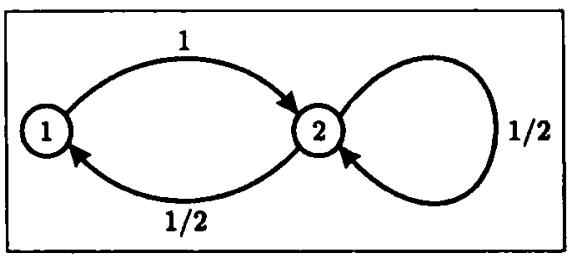
\includegraphics[width=0.8\textwidth]{images/chunk1_5ea8e28f6dd3630e797df891f76f3a7ba5a791ea000aaf358818d8f672052eb1.jpg}
\caption{Transition probabilities of the Markov chain in Exercise \ref{exr:period-two-state}}
\label{fig:exr-5-25}
\end{figure}

\begin{Proposition}
\label{prp:recurrence-type-invariant}
Suppose that $i, j\in S$ and $i \leftrightarrow j$. Show that

\begin{enumerate}
\item $i$ is transient if and only if $j$ is;
\item $i$ is recurrent if and only if $j$ is;
\item $i$ is null-recurrent if and only if $j$ is;
\item $i$ is positive-recurrent if and only if $j$ is;
\item $i$ is periodic if and only if $j$ is, in which case $d(i) = d(j)$;
\item $i$ is ergodic if and only if $j$ is.
\end{enumerate}
\end{Proposition}

\begin{Exercise}
\label{exr:recurrent-implies-intercommunicate}
Show that the following modification of 2) above is true: If $i$ is recurrent and $i \to j$, then $j \to i$. Deduce that if $i$ is recurrent and $i \to j$, then $j$ is recurrent and $j \leftrightarrow i$.

\begin{hint}
Is it possible for a chain starting from $i$ to visit $j$ and then never return to $i$? Is such a situation possible when $i$ is a recurrent state?
\end{hint}
\end{Exercise}

\begin{Solution}
Suppose $i$ is recurrent and $i \to j$, but $j \not\to i$. This means there is a positive probability of reaching $j$ from $i$, but once at $j$, the probability of returning to $i$ is zero.
Let $A$ be the event that the chain reaches $j$ and never returns to $i$. Since $i \to j$ and $j \not\to i$, $P(A \mid \xi_0 = i) > 0$.
However, if $i$ is recurrent, the probability of never returning to $i$ must be zero, i.e., $P(\text{no return to } i \mid \xi_0 = i) = 0$.
This is a contradiction. Thus we must have $j \to i$, so $i \leftrightarrow j$.
By Proposition \ref{prp:recurrence-type-invariant}, since $i$ is recurrent and $i \leftrightarrow j$, $j$ must also be recurrent.
\end{Solution}

The following result describes how the state space $S$ can be partitioned into a countable sum of classes. One of these classes consists of all transient states. Each of the other classes consists of interconnecting recurrent states. If the chain enters one of the classes of second type, it will never leave it. However, if the chain enters the class of transient states, it will eventually leave it (and so never return to it). We begin with a definition.

\begin{Definition}[Closed and irreducible sets]
\label{def:closed-irreducible}
Suppose that $\xi_n, n\in\mathbb{N}$, is a Markov chain on a countable state space $S$.

\begin{enumerate}
\item A set $C \subset S$ is called closed if once the chain enters $C$ it will never leave it, i.e.

\begin{align}
P(\xi_k \in S\setminus C \text{ for some } k \geq n \mid \xi_n \in C) = 0. \tag{5.45}
\end{align}

\item A set $C \subset S$ is called irreducible if any two elements $i, j$ of $C$ intercommunicate, i.e. for all $i, j\in C$ there exists an $n\in\mathbb{N}$ such that $p_n(j \mid i) > 0$.
\end{enumerate}
\end{Definition}

\begin{Theorem}
\label{thrm:state-space-decomposition}
Suppose that $\xi_n, n\in\mathbb{N}$, is a Markov chain on a countable state space $S$. Then

\begin{align}
S = T \cup \bigcup_{j=1}^N C_j, \text{ (disjoint sum)}, \tag{5.46}
\end{align}

where $T$ is the set of all transient states in $S$ and each $C_j$ is a closed irreducible set of recurrent states.
\end{Theorem}

\begin{Exercise}
\label{exr:closed-characterization}
Suppose that $\xi_n, n\in\mathbb{N}$, is a Markov chain on a countable state space $S$. Show that a set $C \subset S$ is closed if and only if $p(j \mid i) = 0$ for all $i\in C$ and $j\in S\setminus C$.

\begin{hint}
One implication is trivial. For the other one use the countable additivity of the measure $P$.
\end{hint}
\end{Exercise}

\begin{Solution}
($\Rightarrow$) Suppose $C$ is closed. By (5.45), $P(\xi_1 \in S \setminus C \mid \xi_0 = i) = 0$ for any $i \in C$.
This can be written as $\sum_{j \in S \setminus C} p(j \mid i) = 0$.
Since $p(j \mid i) \geq 0$, this implies $p(j \mid i) = 0$ for all $j \in S \setminus C$ and $i \in C$.
($\Leftarrow$) Suppose $p(j \mid i) = 0$ for all $i \in C, j \in S \setminus C$.
We want to show that if $\xi_0 \in C$, then $P(\xi_k \in S \setminus C \text{ for some } k \geq 1 \mid \xi_0 \in C) = 0$.
By subadditivity, it suffices to show $P(\xi_k \in S \setminus C \mid \xi_0 = i) = 0$ for all $k \geq 1, i \in C$.
For $k=1$, $P(\xi_1 \in S \setminus C \mid \xi_0 = i) = \sum_{j \in S \setminus C} p(j \mid i) = 0$.
Assume it holds for $k$. Then
\[
P(\xi_{k+1} \in S \setminus C \mid \xi_0 = i) = \sum_{s \in S} P(\xi_{k+1} \in S \setminus C \mid \xi_k = s) P(\xi_k = s \mid \xi_0 = i).
\]
If $s \in C$, $P(\xi_{k+1} \in S \setminus C \mid \xi_k = s) = 0$.
If $s \in S \setminus C$, $P(\xi_k = s \mid \xi_0 = i) = 0$ by the induction hypothesis.
Thus the sum is zero for all $k$.
\end{Solution}

\section{Long-Time Behaviour of Markov Chains: General Case}
\label{sec:long-time-general}

For convenience we shall denote the countable state space $S$ by $\{1,2,3,\cdots\}$ when $S$ is an infinite set and by $\{1,2,\cdots,n\}$ when $S$ is finite.

\begin{Proposition}
\label{prp:limit-implies-invariant}
Let $P = [p(j \mid i)]$ be the transition matrix of a Markov chain with state space $S$. Suppose that for all $i,j\in S$

\begin{align}
\lim_{n\to\infty} p_n(j \mid i) =: \pi_j. \tag{5.47}
\end{align}

(In particular, the limit is independent of $i$.) Then

\begin{enumerate}
\item $\sum_j \pi_j \leq 1$;
\item $\sum_i p(j \mid i) \pi_i = \pi_j$;
\item either $\sum_j \pi_j = 1$, or $\pi_j = 0$ for all $j\in S$.
\end{enumerate}
\end{Proposition}

\begin{Proposition}
\label{prp:invariant-measure}
Let $P = [p(j \mid i)]$ be the transition matrix of a Markov chain with state space $S$. Suppose that for all $i,j\in S$

\begin{align}
\lim_{n\to\infty} p_n(j \mid i) =: \pi_j. \tag{5.47}
\end{align}

Then the vector $\pi = (\pi_j)_{j\in S}$ satisfies $\pi = P^T \pi$, i.e.,

\begin{align}
\sum_{i\in S} p(j \mid i) \pi_i = \pi_j \quad \text{for all } j\in S. \tag{5.65}
\end{align}
\end{Proposition}

\begin{Theorem}
\label{thrm:poisson-binomial}
Suppose that $a \geq 1$ is a natural number. Consider a random walk on $S = \{0,1,\cdots,a\}$ with absorbing barriers at 0 and $a$, and with probability $p$ of moving to the right and probability $q = 1-p$ of moving to the left from any of the states $1,\ldots,a-1$. Hence, our random walk is a Markov chain with transition probabilities

\begin{align}
p(j \mid i) = \begin{cases}
p, & \text{if } 1 \leq i \leq a-1, j = i+1, \\
q, & \text{if } 1 \leq i \leq a-1, j = i-1, \\
1, & \text{if } i = j = 0 \text{ or } i = j = a, \\
0, & \text{otherwise}.
\end{cases}
\end{align}

Find, (a) all invariant measures (there may be just one), (b) the probability of hitting the right-hand barrier prior to hitting the left-hand one.

\begin{hint}
For (a) recall Exercise \ref{exr:invariant-measures-finite} and for (b) Exercise \ref{exr:branching-binomial-poisson}.
\end{hint}
\end{Theorem}

\begin{Exercise}
\label{exr:dice-maximum}
Ian plays a fair game of dice. After the $n$th roll of a die he writes down the maximum outcome $\xi_n$ obtained so far. Show that $\xi_n$ is a Markov chain and find its transition probabilities.

\begin{hint}
$\xi_{n+1} = \max\{\xi_n, X_{n+1}\}$, where $X_k$ is the outcome of the $k$th roll.
\end{hint}
\end{Exercise}

\begin{Solution}
Let $X_n$ be the outcome of the $n$-th roll. $X_n$ are i.i.d. random variables with $P(X_n = k) = 1/6$ for $k \in \{1, \dots, 6\}$.
The maximum outcome after $n+1$ rolls is $\xi_{n+1} = \max\{\xi_n, X_{n+1}\}$. Since $X_{n+1}$ is independent of $X_1, \dots, X_n$, it is also independent of $\xi_n$. Thus, the value of $\xi_{n+1}$ depends only on $\xi_n$ and the independent roll $X_{n+1}$, which proves that $\xi_n$ is a Markov chain.
The state space is $S = \{1, \dots, 6\}$. The transition probabilities $p(j \mid i) = P(\xi_{n+1} = j \mid \xi_n = i)$ are:
- if $j < i$, $p(j \mid i) = 0$ (the maximum cannot decrease).
- if $j = i$, then $X_{n+1} \leq i$, so $p(i \mid i) = P(X_{n+1} \leq i) = i/6$.
- if $j > i$, then $X_{n+1} = j$, so $p(j \mid i) = P(X_{n+1} = j) = 1/6$.
In summary,
\[
p(j \mid i) = \begin{cases} i/6 & \text{if } j=i \\ 1/6 & \text{if } j > i \\ 0 & \text{otherwise} \end{cases}
\]
for $i, j \in \{1, \dots, 6\}$.
\end{Solution}

\begin{Exercise}
\label{exr:pyramid-maximum}
Analyse the Markov chain described in Exercise \ref{exr:dice-maximum}, but with fair die replaced by a fair pyramid.

\begin{hint}
A pyramid has four faces only.
\end{hint}
\end{Exercise}

\begin{Solution}
The analysis is identical to Exercise \ref{exr:dice-maximum}, but with a state space $S = \{1, 2, 3, 4\}$ and probabilities based on 4 faces. The transition probabilities are
\[
p(j \mid i) = \begin{cases} i/4 & \text{if } j=i \\ 1/4 & \text{if } j > i \\ 0 & \text{otherwise} \end{cases}
\]
for $i, j \in \{1, 2, 3, 4\}$.
\end{Solution}

\begin{Exercise}
\label{exr:random-walk-absorbing}
Consider a random walk on $S = \{0,1,\ldots,a\}$ with absorbing barriers at 0 and $a$, and with probability $p$ of moving to the right and probability $q = 1-p$ of moving to the left from any of the states $1,\ldots,a-1$. Find the probability of hitting the right-hand barrier before the left-hand one.

\begin{hint}
Use the result from Proposition \ref{prp:hitting-probability} or solve directly using recurrence relations.
\end{hint}
\end{Exercise}

\begin{Solution}
Let $h_i$ be the probability of hitting $a$ before 0 starting from state $i$. By the law of total probability,
\[
h_i = p h_{i+1} + q h_{i-1} \quad \text{for } 1 \leq i \leq a-1,
\]
with boundary conditions $h_0 = 0$ and $h_a = 1$.
The general solution to this linear difference equation depends on whether $p=q$.
If $p \neq q$, the solution is $h_i = A + B(q/p)^i$. Applying the boundary conditions:
$h_0 = A + B = 0 \Rightarrow B = -A$.
$h_a = A(1 - (q/p)^a) = 1 \Rightarrow A = \frac{1}{1 - (q/p)^a}$.
Thus $h_i = \frac{1 - (q/p)^i}{1 - (q/p)^a}$.
If $p = q = 1/2$, the solution is $h_i = A + Bi$.
$h_0 = A = 0$.
$h_a = Ba = 1 \Rightarrow B = 1/a$.
Thus $h_i = i/a$.
These results match Proposition \ref{prp:hitting-probability}.
\end{Solution}

\begin{Proposition}[Hitting Probability for Random Walk]
\label{prp:hitting-probability}
Consider a random walk on $S = \{0,1,\ldots,a\}$ with absorbing barriers at 0 and $a$, and with probability $p$ of moving to the right and probability $q = 1-p$ of moving to the left from any of the states $1,\ldots,a-1$. Let $h_i$ be the probability of hitting $a$ before 0 starting from state $i$.

Then for $p \neq q$:
\[
h_i = \frac{1 - (q/p)^i}{1 - (q/p)^a},
\]
and for $p = q = 1/2$:
\[
h_i = \frac{i}{a}.
\]
\end{Proposition}

\begin{Exercise}
\label{exr:ergodicity-queuing}
Prove that if there exists an invariant measure for the Markov chain in Exercise \ref{exr:queuing}, then $\lambda' := \sum_{j=0}^\infty j q_j' < 1$. Assuming that the converse is also true, conclude that the chain is ergodic if and only if $\lambda' < 1$. Show that if such an invariant measure exists, then it is unique.

\begin{hint}
Suppose that $\pi = \sum_{j=0}^\infty \pi_j \delta_j$ is an invariant measure. Write down an infinite system of linear equations for $\pi_j$. If you don't know how to follow, look at the solution.
\end{hint}
\end{Exercise}

\begin{Solution}
Let $\pi = (\pi_0, \pi_1, \dots)$ be an invariant distribution. Then $\pi = P^T \pi$.
For the queuing model, the drift at state $i > 0$ is $E[\xi_{n+1} - \xi_n \mid \xi_n = i] = E[Z_n - Y_n] = \lambda - p$.
If an invariant distribution exists, the average drift must be zero:
\[
0 = \sum_{i=0}^\infty \pi_i E[\xi_{n+1} - \xi_n \mid \xi_n = i] = \pi_0 E[Z_n] + \sum_{i=1}^\infty \pi_i (\lambda - p) = \pi_0 \lambda + (1 - \pi_0)(\lambda - p).
\]
This simplifies to $0 = \lambda - (1 - \pi_0) p$, or $\lambda/p = 1 - \pi_0$.
Since $\pi_0 > 0$ for a stable queue, we must have $\lambda/p < 1$, or $\lambda < p$.
If we identify $\lambda' = \lambda/p$ (assuming the unit time is normalized), the condition is $\lambda' < 1$.
The uniqueness follows from the fact that for an irreducible Markov chain, if an invariant distribution exists, it is unique.
\end{Solution}

\section{Long-Time Behaviour of Markov Chains with Finite State Space}

As we have seen above, the existence of the $\pi_j$ plays a very important role in the study of invariant measures. In what follows we shall investigate this question in the case when the state space $S$ is finite.

\begin{Proof}[Proof of Theorem \ref{thrm:finite-state-convergence}]
Denote the matrix $P^{n_0} = [p_{n_0}(j \mid i)]$ by $Q = [q(j \mid i)]$. Then the process $\eta_k = \xi_{kn_0}$, $k \in \mathbb{N}$, is a Markov chain on $S$ with transition probability matrix $Q$ satisfying (5.54) with $n_0$ equal to $1$. Note that $p_{kn_0}(j \mid i) = q_k(j \mid i)$ due to the Chapman--Kolmogorov equations. Suppose that the properties (5.55)--(5.56) hold true for $Q$. In particular, $\lim_{k \to \infty} p_{kn_0}(j \mid i) = \pi_j$ exists and is independent of $i$. We claim that they are also true for the original matrix $P$. Obviously, one only needs to check condition (5.55). The Chapman--Kolmogorov equations (and the fact that $S$ is finite) imply that for any $r = 1, \cdots, n_0 - 1$
\[
\begin{aligned}
p_{kn_0+r}(j \mid i) &= \sum_{s \in S} p_{kn_0}(j \mid s) p_r(s \mid i) \to \sum_{s \in S} \pi_j p_r(s \mid i) \\
&= \pi_j \sum_{s \in S} p_r(s \mid i) = \pi_j.
\end{aligned}
\]

Therefore, by a simple result in calculus, according to which, if for a sequence $a_n$, $n \in \mathbb{N}$, there exists a natural number $n_0$ such that for each $r \in \{0, 1, \cdots, n_0-1\}$ the limit $\lim_{k \to \infty} a_{kn_0+r}$ exists and is $r$-independent, then the sequence $a_n$ is convergent to the common limit of those subsequences, we infer that (5.55) is satisfied.

In what follows we shall assume that (5.54) holds with $n_0 = 1$. Let us put $p_0(j \mid i) = \delta_{ji}$ and for $j \in S$
\[
m_n(j) := \min_{i \in S} p_n(j \mid i), \quad M_n(j) := \max_{i \in S} p_n(j \mid i).
\]

Observe that $M_0(j) = 1$ and $m_0(j) = 0$ for all $j \in S$. From the Chapman-Kolmogorov equations it follows that the sequence $M_n(j)$, $n \in \mathbb{N}$, is decreasing, while the sequence $m_n(j)$, $n \in \mathbb{N}$, is increasing. Indeed, since $\sum_k p(k \mid i) = 1$,
\[
\begin{aligned}
p_{n+1}(j \mid i) &= \sum_{k \in S} p_n(j \mid k) p(k \mid i) \\
&\geq \min_k p_n(j \mid k) \sum_{k \in S} p(k \mid i) = \min_k p_n(j \mid k) = m_n(j).
\end{aligned}
\]

Hence, by taking the minimum over all $i \in S$, we arrive at
\[
m_{n+1}(j) = \min_i p_{n+1}(j \mid i) \geq m_n(j).
\]

Similarly,
\[
\begin{aligned}
p_{n+1}(j \mid i) &= \sum_{k \in S} p_n(j \mid k) p(k \mid i) \\
&\leq \max_k p_n(j \mid k) \sum_{k \in S} p(k \mid i) = \max_k p_n(j \mid k) = M_n(j).
\end{aligned}
\]

Hence, by taking the maximum over all $i \in S$, we obtain
\[
M_{n+1}(j) = \max_i p_{n+1}(j \mid i) \leq M_n(j).
\]

Since $M_n(j) \geq m_n(j)$, the sequences $M_n(j)$ and $m_n(j)$ are bounded from below and from above, respectively. As a consequence, they both have limits. To show that the limits coincide we shall prove that
\[
\lim_{n \to \infty} (M_n(j) - m_n(j)) = 0. \tag{5.57}
\]

For $n \geq 0$ we have
\[
p_{n+1}(j \mid i) = \sum_{s \in S} p_n(j \mid s) p(s \mid i) \tag{5.58}
\]
\[
= \sum_{s \in S} p_n(j \mid s) [p(s \mid i) - \varepsilon p_n(s \mid j)] + \varepsilon \sum_{s \in S} p_n(j \mid s) p_n(s \mid j)
\]
\[
= \sum_{s \in S} p_n(j \mid s) [p(s \mid i) - \varepsilon p_n(s \mid j)] + \varepsilon p_{2n}(j \mid j)
\]
by the Chapman--Kolmogorov equations. The expression in square brackets is $\geq 0$. Indeed, by assumption (5.54), $p(s \mid i) \geq \varepsilon$ and $p_n(s \mid j) \leq 1$. Therefore,
\[
p_{n+1}(j \mid i) \geq \min_{s \in S} p_n(j \mid s) \sum_{s \in S} [p(s \mid i) - \varepsilon p_n(s \mid j)] + \varepsilon p_{2n}(j \mid j) \tag{5.59}
\]
\[
= (1 - \varepsilon) m_n(j) + \varepsilon p_{2n}(j \mid j).
\]

By taking the minimum over $i \in S$, we arrive at
\[
m_{n+1}(j) \geq (1 - \varepsilon) m_n(j) + \varepsilon p_{2n}(j \mid j). \tag{5.60}
\]

Recycling the above argument, we obtain a similar inequality for the sequence $M_n(j)$:
\[
M_{n+1}(j) \leq (1 - \varepsilon) M_n(j) + \varepsilon p_{2n}(j \mid j). \tag{5.61}
\]

Thus, by subtracting (5.60) from (5.61) we get
\[
M_{n+1}(j) - m_{n+1}(j) \leq (1 - \varepsilon) (M_n(j) - m_n(j)). \tag{5.62}
\]

Hence, by induction
\[
M_n(j) - m_n(j) \leq (1 - \varepsilon)^n, \quad n \in \mathbb{N}.
\]

This proves (5.57). Denote by $\pi_j$ the common limit of $M_n(j)$ and $m_n(j)$. Then (5.55) follows from (5.57). Indeed, if $i, j \in S$, then
\[
m_n(j) \leq p_n(j \mid i) \leq M_n(j).
\]

To prove that $\pi_j > 0$ let us recall that $m_n(j)$ is an increasing sequence and $m_1(j) \geq \varepsilon$ by (5.54). We infer that $\pi_j \geq \varepsilon$. $\square$
\end{Proof}

\begin{Exercise}
\label{exr:exponential-convergence}
Show that $p_n(j \mid i) \to \pi_j$ at an exponential rate.

\begin{hint}
Recall that $m_n(j) \leq \pi_j \leq M_n(j)$ and use (5.57).
\end{hint}
\end{Exercise}

\begin{Solution}
From the proof of Theorem \ref{thrm:finite-state-convergence}, it is shown that the difference between the maximum and minimum values of $p_n(j \mid \cdot)$ decreases geometrically. Specifically,
\[
M_{k n_0}(j) - m_{k n_0}(j) \leq (1-\varepsilon)^k
\]
for some $\varepsilon > 0$. Since $m_n(j) \leq p_n(j \mid i) \leq M_n(j)$ and $m_n(j) \leq \pi_j \leq M_n(j)$, we have
\[
|p_{k n_0}(j \mid i) - \pi_j| \leq (1-\varepsilon)^k = [(1-\varepsilon)^{1/n_0}]^{k n_0}.
\]
Setting $\alpha = (1-\varepsilon)^{1/n_0} < 1$, we see that $|p_n(j \mid i) - \pi_j| \leq C \alpha^n$ for some constant $C$, which demonstrates an exponential rate of convergence.
\end{Solution}

The above proves the following important result.

\begin{Theorem}[Finite State Space Convergence]
\label{thrm:finite-state-convergence}
Suppose that $S$ is finite and the transition matrix $P = [p(j \mid i)]$ of a Markov chain on $S$ satisfies the condition

\begin{align}
\exists n_0 \in \mathbb{N} \exists \varepsilon > 0: p_{n_0}(j \mid i) \geq \varepsilon, \quad i, j \in S. \tag{5.54}
\end{align}

Then, the following limit exists for all $i, j \in S$ and is independent of $i$:

\begin{align}
\lim_{n \to \infty} p_n(j \mid i) = \pi_j. \tag{5.55}
\end{align}

The numbers $\pi_j$ satisfy

\begin{align}
\pi_j > 0, \quad j \in S \quad \text{and} \quad \sum_{j \in S} \pi_j = 1. \tag{5.56}
\end{align}

Conversely, if a sequence of numbers $\pi_j, j \in S$ satisfies conditions (5.55)-(5.56), then assumption (5.54) is also satisfied.
\end{Theorem}

\begin{Theorem}[Ergodic Finite State Space]
\label{thrm:ergodic-finite}
Suppose that $\xi_n, n \in \mathbb{N}$, is an irreducible aperiodic Markov chain with finite state space $S$. Then $\xi_n$ is ergodic if and only if it has a unique invariant measure.
\end{Theorem}

\begin{Exercise}
\label{exr:invariant-measures-finite}
Investigate the existence and uniqueness of an invariant measure for the Markov chain in Proposition \ref{prp:telephone-is-markov}.

\begin{hint}
Are the assumptions of Theorem \ref{thrm:finite-state-convergence} satisfied?
\end{hint}
\end{Exercise}

\begin{Solution}
The transition matrix is $P = \begin{bmatrix} 1-p & q \\ p & 1-q \end{bmatrix}$. Since $0 < p, q < 1$, all entries of $P$ are strictly positive. Thus, condition (5.54) is satisfied with $n_0 = 1$ and $\varepsilon = \min\{1-p, q, p, 1-q\} > 0$.
By Theorem \ref{thrm:ergodic-finite}, there exists a unique invariant measure for this Markov chain.
\end{Solution}

\begin{Remark}
\label{rem:solve-invariant-directly}
The solution to Exercise \ref{exr:invariant-measures-finite} allows us to find the unique invariant measure by direct methods, i.e. by solving the linear equations (5.79)-(5.80).
\end{Remark}

\begin{Exercise}
\label{exr:find-invariant-limit}
Find the invariant measure from Exercise \ref{exr:invariant-measures-finite} by calculating the limits (5.55).

\begin{hint}
Refer to Solution 5.5.
\end{hint}
\end{Exercise}

\begin{Solution}
From Exercise \ref{exr:find-n-step-transition}, the $n$-step transition probabilities are
\[
p_n(0 \mid 0) = \frac{q}{q+p} + \frac{p}{q+p}(1-p-q)^n \to \frac{q}{q+p},
\]
\[
p_n(0 \mid 1) = \frac{q}{q+p} - \frac{q}{q+p}(1-p-q)^n \to \frac{q}{q+p}.
\]
Thus $\pi_0 = \frac{q}{q+p}$. Similarly, $\pi_1 = \frac{p}{q+p}$. The invariant measure is $\pi = \left( \frac{q}{q+p}, \frac{p}{q+p} \right)$.
\end{Solution}

\begin{Exercise}
\label{exr:finite-state-summary}
For each of the following transition matrices, determine: (a) whether the chain is irreducible, (b) whether it is aperiodic, (c) the invariant distribution (if it exists), (d) whether the chain is ergodic.

\begin{enumerate}
\item $P = \begin{bmatrix} 0.5 & 0.5 \\ 0.5 & 0.5 \end{bmatrix}$
\item $P = \begin{bmatrix} 0 & 1 \\ 1 & 0 \end{bmatrix}$
\item $P = \begin{bmatrix} 0.5 & 0.25 & 0.25 \\ 0 & 0.5 & 0.5 \\ 0 & 0 & 1 \end{bmatrix}$
\end{enumerate}

\begin{hint}
Check the definitions of irreducibility, aperiodicity, and use Theorem \ref{thrm:ergodic-finite}.
\end{hint}
\end{Exercise}

\begin{Solution}
\begin{enumerate}
\item $P = \begin{bmatrix} 0.5 & 0.5 \\ 0.5 & 0.5 \end{bmatrix}$:
(a) Irreducible: All entries are positive, so any state can reach any other.
(b) Aperiodic: $p(1 \mid 1) > 0$.
(c) Invariant distribution: $\pi = (0.5, 0.5)$.
(d) Ergodic: Yes, it is irreducible, aperiodic, and positive recurrent (finite state).
\item $P = \begin{bmatrix} 0 & 1 \\ 1 & 0 \end{bmatrix}$:
(a) Irreducible: Yes.
(b) Periodic: $p_1(1 \mid 1) = 0$, $p_2(1 \mid 1) = 1$, $p_3(1 \mid 1) = 0$. Period $d = 2$.
(c) Invariant distribution: $\pi = (0.5, 0.5)$.
(d) Ergodic: No (not aperiodic).
\item $P = \begin{bmatrix} 0.5 & 0.25 & 0.25 \\ 0 & 0.5 & 0.5 \\ 0 & 0 & 1 \end{bmatrix}$:
(a) Not irreducible: State 3 is absorbing and cannot reach states 1 or 2.
(b) Aperiodic: All diagonal entries are positive.
(c) Invariant distribution: $\pi = (0, 0, 1)$.
(d) Not ergodic: Not irreducible.
\end{enumerate}
\end{Solution}

